\documentclass[12pt,a4paper,openany,oneside]{book}

\usepackage[a4paper,margin=2cm]{geometry}


\usepackage{hyperref}
\usepackage[english]{babel}
\usepackage{amsfonts}

\usepackage[utf8x]{inputenc}
\usepackage{graphicx}
\usepackage{subcaption}
\usepackage[font=small,labelfont=bf,tableposition=top]{caption}

\usepackage{listings}
\usepackage{courier}
\lstset{
       language=C++,
       basicstyle=\footnotesize\ttfamily,
       numbers=left,
       numberstyle=\tiny,
       numbersep=5pt,
       tabsize=5,
       extendedchars=true,
       breaklines=true,
       keywordstyle=\textbf,
       stringstyle=\color{white}\ttfamily,
       showspaces=false,
       showtabs=false,
       xleftmargin=17pt,
       framexleftmargin=17pt,
       framexrightmargin=5pt,
       framexbottommargin=4pt,
       showstringspaces=false,
       escapeinside={(*@}{@*)}
 }

 \addto\captionsenglish{ \renewcommand{\lstlistingname}{Algorithm}}

\setcounter{tocdepth}{3} \setcounter{secnumdepth}{3}

\usepackage{tikz}
\usepackage{amsmath}
\usepackage{framed}

\begin{document}

\begin{titlepage}
\centering
\includegraphics[width=2.434cm,height=2.565cm]{images/university_logo.png}

\bigskip

{\Large \textbf{UNIVERSITÀ DI CATANIA}}

{\scshape
\large
Dipartimento di Matematica e Informatica
}

{\scshape
\normalsize
Laurea Triennale in Informatica
}

\bigskip


\hrule


\bigskip


\bigskip


\bigskip


\bigskip

{\itshape
\large
Matteo Galletta
\par}


\bigskip


\bigskip


\bigskip


\bigskip

{\centering
\Large
Minimum Weight Vertex Cover Problem
\par}


\bigskip


\bigskip


\bigskip


\bigskip


\bigskip


\bigskip


\begin{minipage}[b]{8 cm}
\hrule

\bigskip

{\centering\scshape
Artificial Intelligence Project
\par}


\bigskip

\hrule
\end{minipage}
\bigskip


\bigskip


\bigskip


\bigskip


\bigskip


\bigskip


\bigskip


\bigskip


\bigskip


\bigskip


\bigskip

{\raggedleft
Professors: Mario Francesco Pavone \\
Vincenzo Cutello
\par}


\bigskip


\bigskip


\bigskip


\bigskip

\hrule

\bigskip

{\centering
Academic Year 2024 - 2025
\par}
\end{titlepage}

\bibliographystyle{unsrt}
\title{Minimum Weight Vertex Cover Problem}
\author{Matteo Galletta}

\tableofcontents

\chapter{Introduction}

\section{Problem}

Given a problem instance $(G, \omega)$, where $G$ is a undirected graph $G(V, E)$ and $\omega: V \to \mathbb{R}^{+}$ a function that associates a positive weight value $\omega(v)$ to each vertex $v \in V$, the Minimum Weight Vertex Cover can formally be defined as follows:

\[ \textbf{minimize} \quad \omega(S) = \sum_{v \in S} \omega(v), \quad S \in V \]

{
	\centering
	such that $\forall (v_i, v_j) \in E, v_i \in S \lor v_j \in S$.
}

Note that the MWVC is a NP-complete problem.

\section{Proposed Solution and Motivation}

This project implements a solution to the MWVC problem using a \emph{Genetic Algorithm (GA) with one-point crossover and k-tournament selection}.
\par
The chosen algorithm facilitates parallel computing compared to Tabu Search, as well as allowing to reduce the risk of the local optima stagnation. Also, Branch-and-Bound has limitations concerning the problem size, while Genetic Algorithms are suitable for NP-Hard problems such as MWVC.
\par
Regarding the chosen Genetic Algorithm variation, even though it is not immediate to state whether one-point crossover will achieve better results over uniform crossover without prior testing, it has been widely proved that k-tournament selection outperforms roulette wheel in most scenarios \cite{ktournament-vs-wheeler}.

\chapter{Genetic Algorithms}

\section{Behaviour and Structure}

Genetic Algorithms (GAs) are a class of evolutionary algorithms inspired by the principles of natural selection. They operate by iteratively evolving a population of potential solutions towards an optimal or near-optimal state. The process unfolds as follows:

\begin{description}

	\item[Initialization] An initial population of candidate solutions is randomly generated.

	\item[Evaluation] Each individual in the population is evaluated based on a predefined fitness function, which quantifies its quality or suitability with respect to the problem at hand.

	\item[Selection] A subset of individuals are selected from the populations. The chosen individuals are selected as parents of the following population. Selection is based on fitness, with fitter individuals having a higher probability of being chosen.

	\item[Crossover] Using crossover, selected parents genetic material are combined to create offspring.
	
	\item[Mutation] With a certain probability, random mutations are introduced into the offspring. This is called mutation and it helps to maintain diversity within the population and prevents premature convergence towards suboptimal solutions.
	
	\item[Replacement] This newly generated population replaces the old one.
	
\end{description}

The cycles of evaluation, selection, crossover, mutation, and replacement are repeated until a halting criteria is satisfied.

\section{k-Tournament Selection}

The selection algorithm for the proposed solution is \emph{k-tournament}.
This algorithm involves running several "tournaments" among k individuals chosen at random from the population, until the desired amount of population is reached. Each tournament selects the best amongst the k selected individuals.

The tournament size $k$ can be adjusted to balance exploration and exploitation. Smaller k introduces more diversity, while larger k focuses more on exploiting fittest individuals.
Given a population of $n$ individuals:
\begin{enumerate}
  \item[] $k=1:$ \quad selection is random, there is no preference based on fitness
  \item[] $k=n:$ \quad the fittest individuals are always selected 
\end{enumerate}

\begin{framed}
\begin{lstlisting}[caption=k-tournament selection]
function k-tournament(population, k, n)
	new_population = []
	while new_population.size < n
		selected = []
		while selected.size < k
			individual = (*@\textit{random element from population}@*)
			selected.push(individual)
		end
		new_population.push(best(selected))
	end
	return new_population
end
\end{lstlisting}
\end{framed}


\section{Single-Point Crossover}

The simplest form of crossover is the single-point crossover, where a random crossover point is selected and the genetic material is exchanged between the parents at that point.

\begin{framed}
\begin{lstlisting}[caption=Single-point crossover]
function single-point-crossover(parent1, parent2)
	i = (*@\textit{random integer in [0..n-1]}@*)
	offspring1 = parent1[0..i] + parent2[i+1..n-1]
	offspring2 = parent2[0..i] + parent1[i+1..n-1]
	return offspring1, offspring2
end
\end{lstlisting}
\end{framed}

\section{Bit-Flip Mutation}

Mutation is a genetic operator that introduces random changes in the offspring. The simplest form of mutation is the bit-flip mutation, where a bit has a probability $p$ of being flipped.

\begin{framed}
\begin{lstlisting}[caption=Bit-flip mutation]
function bit-flip-mutation(offspring, p)
	for i in 0..n-1
		if random() < p
			offspring[i] = 1 - offspring[i]
		end
	end
	return offspring
end
\end{lstlisting}
\end{framed}







\chapter{Implementation}

\section{DEAP Framework}

\par
The chosen framework for the implementation is DEAP \cite{DEAP_JMLR2012}.
DEAP (Distributed Evolutionary Algorithms in Python) is a Python library that excels at rapid prototyping and testing of ideas, making the tool ideal for the project.

\section{Gene Representation}

The gene representation is a binary string, where each bit represents the presence of a vertex in the solution.
The length of the string is equal to the number of vertices in the graph.
The weight of the vertex is stored in a separate list, where the index corresponds to the vertex index.

\begin{figure}[ht]
\centering
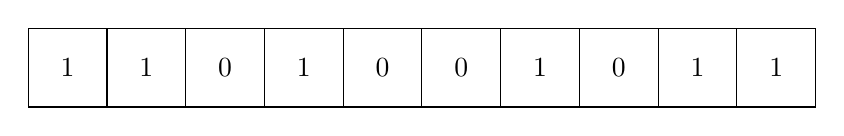
\begin{tikzpicture}
	\foreach \i in {1,2,4,7,9,10} {
		\draw (\i,0) rectangle (\i+1,1);
		\node at (\i+0.5,0.5) {1};
		}
	\foreach \i in {3,5,6,8} {
		\draw (\i,0) rectangle (\i+1,1);
		\node at (\i+0.5,0.5) {0};
	}
\end{tikzpicture}
\caption{Example of a MWVC gene representation}
\end{figure}

\section{Fitness Function}

The fitness function for the Minimum Weight Vertex Cover problem calculates the weight of the solution by summing the weights of the vertices present in the solution.
Additionally, it imposes a penalty for each edge that is not covered by the vertices in the solution, ensuring that the fitness value is higher for incomplete solutions.
The penalty function (or a similar alternative) is mandatory since we're using a direct gene representation that could create invalid configurations of uncovered vertices.

\begin{framed}
\begin{lstlisting}[caption=Fitness function]
function fitness(individual)
	f = 0
	for i in 0..n-1
		if individual[i] == 1
			f = f + vertex_weight[i]
		end
	end

	for edge in graph.edges
		if individual[edge.from] == 0 and individual[edge.to] == 0
			f = f + penalty
		end
	end
	return f
end
\end{lstlisting}
\end{framed}

The objective function is the same but with a penalty of zero, and it returns $\text{NULL}$ if the solution is invalid (i.e. there are uncovered edges).



\section{Performance Metrics}

In order to evaluate the performance of the algorithm, it is necessary to define a set of metrics to evaluate the quality of the solution and the performance of the algorithm.

The most important one is the fitness, as well as the objective (that does not include the penalties). Another metric to optimize is the number of evaluations, as it is a direct measure of the computational cost of the algorithm.

The execution time is not considered as a metric as it is highly dependent on the hardware and software environment.

It would be useful to include an optimality metric representing the difference between the best known solution and the solution found by the algorithm, but this information is not easily computable as the problem is NP-hard.

\section{Parameters}

Genetic Algorithms have a set of parameters that need to be tuned in order to achieve the best performance.

The following is the list of the meta-parameters configurable in the implementation:

\begin{itemize}
	\item \textbf{Population size} (\texttt{POPULATION\_SIZE}): the number of individuals in the population.
	\item \textbf{Crossover probability} (\texttt{CXPB}): the probability of crossover.
	\item \textbf{Mutation probability} (\texttt{MUTPB}): the probability of mutation.
	\item \textbf{k-tournament selection size} (\texttt{K\_TOURNAMENT}): the size $k$ of the tournament in the k-tournament selection.
	\item \textbf{Number of generations} (\texttt{NUMBER\_OF\_GENERATIONS}): the number of generations the algorithm will run.
\end{itemize}

The problem of finding the best parameters is an optimization problem itself, and it is possible to use a meta-heuristic algorithm to find the best parameters, such as a Genetic Algorithm \cite{meta-heuristic}. This is out of the scope of this project even though it could be an interesting future development.

\section{Benchmarking Flow}

This paragraph describes the flow of the benchmarking process. The goal of the benchmarking process is to test the algorithm with a fixed parameters combination over different graph instances to extract the metrics and evaluate the performance of the algorithm. The parameters are chosen based on the literature and are discussed in the chapter 4.

The process is divided into the following steps:

\begin{enumerate}
	\item \textbf{Load the graphs}: the problem instances for testing are loaded from the files.
	\item \textbf{Compute graphs properties}: for each graph a set of properties are computed, such as the number of vertices, the number of edges and the density.
	\item \textbf{Create the DEAP structures}: the DEAP structures are created, including the individuals, the population and the evaluation function.
	\item \textbf{Run the algorithm}: the algorithm is executed with the set parameters over the graph instances.
	\item \textbf{Save the results}: the results are saved to a multiple files in JSON format for further analysis.
	\item \textbf{Analyze the results}: the results are analyzed to extract the metrics and evaluate the performance of the algorithm.
\end{enumerate}

Every step, except the last one, is executed within a Python script with configurable parameters. The last step is performed using a Jupyter Notebook for a faster and more interactive analysis.

The benchmarking process is repeated iteratively over different parameters combinations to find the best configuration for the algorithm.


\chapter{Results}

\section{Introduction}

As previously stated, this chapter describes the process of tuning the parameters of the genetic algorithm and the results obtained from the experiments.

\section{Iteration 1: Default Parameters}

This first iterations consists of the most basic configuration of the genetic algorithm with literature defaults \cite{literature-defaults}.

\begin{table}[h]
    \centering
    \begin{tabular}{|c c|}
        \hline
        \textbf{Parameter} & \textbf{Value} \\
        \hline
        POPULATION\_SIZE & 100 \\
        CXPB & 0.5 \\
        MUTPB & 0.2 \\
        K\_TOURNAMENT & 3 \\
        NUMBER\_OF\_GENERATIONS & 1 000 000 \\
        \hline
    \end{tabular}
    \caption{Parameters for Iteration 1}
    \label{tab:iteration1_parameters}
\end{table}

The currently implemented genetic algorithm struggles to find a valid solution for MPI and LPI instances. The evaluation limit makes the algorithm stop before a valid individual is found. The main reason could be the penalty value, which is set to the max weight of the vertices. This is a fixed value that doesn't scale well for higher problem sizes. This gives a hint that the penalty value should be set to a value that is proportional to the problem size. In particular, many different formulas have been used to calculate the penalty value, but none of these have shown any improvement.

The chosen solution is to remove the penalty mechanism and replace it with a repair mechanism that will fix the invalid individuals. It will perform a greedy repair by selecting the vertex with best ratio of covered edges over total weight. This repair mechanism is not perfect, but it's a good compromise between efficiency and accuracy.
This ensures that the genetic algorithm will always return a valid solution, even if it's not the best one.

\begin{lstlisting}[caption=Repair mechanism]

function repair(individual):
    WHILE any edge (u,v) is not covered by individual:
        Find vertex w with lowest (weight/number_of_uncovered_edges_it_covers)
        individual[w] = 1
    RETURN individual
end
\end{lstlisting}

Since the algorithm was now very slow, a compromise was made: the repair mechanism was only applied for the first generation. This way, the genetic algorithm could find a valid solution and then improve it. This is not the best solution, but it's a good compromise between efficiency and accuracy.

The results for the initial iteration are as follows.

\begin{table}[h]
    \centering
    \begin{tabular}{|l l r r|}
        \hline
        \textbf{Problem Class} & \textbf{Test Instance} & \textbf{Average Objective} & \textbf{Average Evaluations} \\
        \hline
        LPI & 10000 & 48052.6 & 20000.0 \\
        MPI & 3000  & 12110.3  & 20000.0 \\
        MPI & 2000  & 6129.4   & 20000.0 \\
        MPI & 750   & 9512.6  & 20000.0 \\
        MPI & 500   & 4849.5   & 20000.0 \\
        SPI & 150   & 1269.5   & 20000.0 \\
        SPI & 120   & 1039.0    & 20000.0 \\
        SPI & 60    & 865.8   & 20000.0 \\
        \hline
    \end{tabular}
    \caption{Results for Iteration 1}
    \label{tab:gen_objective_summary}
\end{table}

\section{Iteration 2: Population Size}

The first parameter to be tuned is the population size. The test is initially performed using a population size of 50, 75, 100, 150, 200 and 400.
The results are compared using the average objective function value since the average number of evaluations would still be capped at 20000.

After performing the tests, it looks like the population size of 400 is the best for every test instance. The improvement is not significant, but it's still better than the other population sizes.

\begin{table}[h!]
    \centering
    \begin{tabular}{|c|c c c c c c c|}
    \hline
    \textbf{Pop. size} & \textbf{50} & \textbf{75} & \textbf{100} & \textbf{125} & \textbf{150} & \textbf{200} & \textbf{400} \\
    \hline
    \textbf{Avg obj} & 10496.7375 & 10472.7875 & 10478.625 & 10445.65 & 10461.3 & 10440.8 & 10406.175 \\
    \hline
    \end{tabular}
    \caption{Average Objective for different Population Sizes}
    \label{table:gen_objective}
\end{table}

This iteration keeps the parameters the same as the precedent iteration, except for the population size which is now set to 400.

The results are as follows.

\begin{table}[h]
    \centering
    \begin{tabular}{|l l r r|}
        \hline
        \textbf{Problem Class} & \textbf{Test Instance} & \textbf{Average Objective} & \textbf{Average Evaluations} \\
        \hline
        LPI & 10000 & 47782.5 & 20000.0 \\
        MPI & 3000  & 11975.2  & 20000.0 \\
        MPI & 2000  & 6085.5   & 20000.0 \\
        MPI & 750   & 9439.5  & 20000.0 \\
        MPI & 500   & 4801.9   & 20000.0 \\
        SPI & 150   & 1264.0   & 20000.0 \\
        SPI & 120   & 1039.0    & 20000.0 \\
        SPI & 60    & 861.8   & 20000.0 \\
        \hline
    \end{tabular}
    \caption{Results for Iteration 2}
    \label{tab:gen_objective_summary}
\end{table}
\FloatBarrier

\section{Iteration 3: Crossover and Mutation Probabilities}

The next parameters to be tuned are the crossover and mutation probabilities. Since these two parameters are closely related, they will be tested together.
The test is performed using a grid search with the following values: 0.01, 0.05 and 0.1 for mutation probability and 0.3, 0.5 and 0.7 for crossover probability.
A bash script is used to run all the tests at once.

The results show that aren't better compared to the previous ones. 
The final choice consists of 0.5 and 0.2 for crossover and mutation probability respectively.

\begin{table}[h]
    \centering
    \begin{tabular}{|c c|}
        \hline
        \textbf{Parameter} & \textbf{Value} \\
        \hline
        POPULATION\_SIZE & 400 \\
        CXPB & \textbf{0.4} \\
        MUTPB & \textbf{0.25} \\
        K\_TOURNAMENT & 3 \\
        NUMBER\_OF\_GENERATIONS & 1 000 000 \\
        \hline
    \end{tabular}
    \caption{Parameters for Iteration 3}
    \label{tab:iteration1_parameters}
\end{table}

The results are the same of the previous iteration since the parameters were not changed, so they are not shown here.

\section{Iteration 4: Tournament Size}

The next parameter to be tuned is the tournament size. The test is performed with the following values: 2, 3, 4, 5.

The results show that the best tournament size are 3 and 4.
Even tough the tournament size of 4 looks better for some test instances, $K=3$ performs better for the majority of the test instances. Another reason to choose the tournament size of 3 is that it allows for a faster convergence, due to its faster selection process.
3 is chosen as tournament size.

The average objective value is the same as the previous iteration, so it's not shown here.

\section{Iteration 5: Number of Generations}

The number of generations is by far the most important parameter to be tuned, as well as the hardest to tune. By now, the genetic algorithm has been tuned to the best of its abilities, and the number of generations was not considered in the previous iterations. This iteration will improve considerably the efficiency of the genetic algorithm, with the downside of getting a slightly less accurate solution.
The best way to tune this parameter is to plot the average objective function value by generation and see when the genetic algorithm converges.

At first glance, the plots show how the problem size doesn't look to depend at all on the number of generations. Figure \ref{fig:performance_plots_it5} shows this behavior. Binding the number of generations to the problem size is not a good idea.

\begin{figure}[h]
    \centering
    \begin{subfigure}{0.32\textwidth}
        \centering
        \includegraphics[width=\linewidth]{../results/5/plots/objective_vs_gen_3000_01.txt.jpg}
        \caption{Test Instance 3000 (n° 1)}
    \end{subfigure}
    \hfill
    \begin{subfigure}{0.32\textwidth}
        \centering
        \includegraphics[width=\linewidth]{../results/5/plots/objective_vs_gen_3000_07.txt.jpg}
        \caption{Test instance 3000 (n° 7)}
    \end{subfigure}
    \hfill
    \begin{subfigure}{0.32\textwidth}
        \centering
        \includegraphics[width=\linewidth]{../results/5/plots/objective_vs_gen_3000_09.txt.jpg}
        \caption{Test instance 3000 (n° 9)}
    \end{subfigure}

    \caption{Objective function value by generation for different test instances}
    \label{fig:performance_plots_it5}
\end{figure}
\FloatBarrier

The remaining option is to dynamically set the number of generations depending on a dynamic convergence criteria. The chosen criteria is to stop the genetic algorithm when the average objective function value doesn't improve for 40 generations.

There could be better criteria, but this one was chosen for its simplicity. This still manages to half the number of generations for most test instances.

\begin{table}[h]
    \centering
    \begin{tabular}{|c c|}
        \hline
        \textbf{Parameter} & \textbf{Value} \\
        \hline
        POPULATION\_SIZE & 400 \\
        CXPB & 0.4 \\
        MUTPB & 0.25 \\
        K\_TOURNAMENT & 3 \\
        NUMBER\_OF\_GENERATIONS & \textbf{dynamic} \\
        \hline
    \end{tabular}
    \caption{Parameters for Iteration 5}
    \label{tab:iteration1_parameters}
\end{table}

The final results are as follows.

\begin{table}[h]
    \centering
    \begin{tabular}{|l l r r|}
        \hline
        \textbf{Problem Class} & \textbf{Test Instance} & \textbf{Average Objective} & \textbf{Average Evaluations} \\
        \hline
        LPI	& 10000	& 47784.5	& 10501.7 \\
        MPI	& 3000	& 12054.5	& 12279.1 \\
        MPI	& 2000	& 6091.0	& 12021.6 \\
        MPI	& 750	& 9460.2	& 16703.0 \\
        MPI	& 500	& 4768.6	& 18637.0 \\
        SPI	& 150	& 1264.0	& 10272.1 \\
        SPI	& 120	& 1038.2	& 10222.2 \\
        SPI	& 60	& 861.8     & 10430.5 \\
        \hline
    \end{tabular}
    \caption{Results for Iteration 5}
    \label{tab:gen_objective_summary}
\end{table}



\chapter*{Conclusion}

The analysis shows how an iterative process can be a solution to find the best parameters for a genetic algorithm implementation.
I found it hard to find a linear path to the solution, but the iterative process helped me to find the best parameters for the genetic algorithm. I learned how this kind of tuning process is very difficult to standardize due to the uniqueness of each problem. I am pround and happy of the results I got, especially regarding the framework created to test and then analyze the results. I think this was the key to succeed in these kinds of experimental projects.

The problem task suggested to run each test ten times and then perform the average of the results. I think this is a good approach to reduce the noise in the results, but I feel that for this algorithm implementation it wasn't enought. It looked like different executions gave too different results, and I think that running the tests more times could have helped to reduce the noise even more, allowing for more accurate results.

Despite the obtained results, I believe it would be interesting to approach the problem using a metaheuristic algorithm, such as the genetic algorithm itself, to solve the problem of finding the best parameters for the genetic algorithm. The iterative process is slow and requires a lot of manual work, while a metaheuristic algorithm could be more challenging and fun.

I really enjoyed working on this project, I think I learned a lot about genetic algorithms and how to tune them. The task problem was clear and having the test instances ready saved me plenty of time. This was my first experimental research project, and the freedom to choose any language and technology I believe was the essence of the project, even though it was a bit challenging to find the best tools to use and I was a little bit lost in the beginning. When looking for literature resources, I found the No Free Lunch Theorem \cite{NFL-theorem}, which left me slightly unsettled but gave me a different approach to the problem. I hope to have the opportunity to work on more projects like this in the future.


\addcontentsline{toc}{chapter}{Conclusion}

\newpage
\addcontentsline{toc}{chapter}{Bibliography}
\bibliography{bibliography}
\end{document}